\documentclass[12pt]{article}
\usepackage{lmodern} % Add the lmodern package to fix missing font shapes
% Use fontspec for Unicode support
\usepackage{fontspec}

% \usepackage[utf8]{inputenc}

%% PACKAGES
% Meta
\usepackage{geometry, color, hyperref, ragged2e, setspace}
%\usepackage{pdflscape} % Produce landscape pages in a (mainly) portrait document.
% Maths
\usepackage{amsmath, amsfonts, unicode-math, bbold}
\setmathfont{latinmodern-math.otf}

% Bibliography
\usepackage[backend=biber, style=apa]{biblatex}
\addbibresource{references.bib}  % This is the file exported from Zotero

% Graphics
\usepackage{graphicx, subcaption}
% Tables
\usepackage{threeparttable, booktabs, caption, dcolumn, threeparttablex, longtable, adjustbox, multirow}
\usepackage{rotating} 
% Lists
\usepackage{enumitem}
\setlist[itemize]{noitemsep}
% Epigraph
\usepackage{epigraph}
% Typesetting
\usepackage{soul} % Break line in underline with \ul
%\usepackage{microtype} % Improve word breaking


%%%%% MINIMAL EXTENSIONS
\RequirePackage[TS1,T1]{fontenc}			%% font encodage
%\RequirePackage{lmodern}					%% latin font
%\RequirePackage{fourier-otf}			    %% Adobe Utopia font
\RequirePackage{textcomp}					%% other symbols
\setlength{\parindent}{20pt}                %% par indent

% Optional: Set a modern font (e.g., Latin Modern or Times New Roman)
\setmainfont{Latin Modern Roman}

%% PACKAGES OPTIONS
% BASE: Penalty to avoid split in footnotes
\interfootnotelinepenalty=10000
% GEOMETRY: Page size
\geometry{left = 1.0in, right = 1.0in, top = 1.0in , bottom = 1.0in}
% HYPERREF : Hyperlink colors
\hypersetup{
	colorlinks = true,
	linkcolor = blue,
	anchorcolor = blue,
	citecolor = blue,
	filecolor = blue,
	urlcolor = blue
}
% AMSMATH : theorems environments
\newtheorem{theorem}{Theorem}
\newtheorem{assumption}{Assumption}
\newtheorem{corollary}[theorem]{Corollary}
\newtheorem{proposition}{Proposition}
\newtheorem{lemma}[theorem]{Lemma}
\newtheorem{conjecture}{Conjecture}
\newenvironment{proof}[1][Proof]{\noindent\textbf{#1.} }{\ \rule{0.5em}{0.5em}}
% AUTHBLK
% \renewcommand\Authands{ and } % Remove the comma before 'and'
% TITLE / AUTHOR /DATE
\usepackage{titling}

\begin{document}

%% Title
\title{Gender (In)equality in England: Occupations, Tasks and Wages\thanks{
We are grateful to <Names>, as well as to audiences at the <Conferences> and seminar participants at <Seminars> for useful comments and suggestions. 
This work was supported by <Grants>.
}}

%% Authors
\author{German Pulido\thanks{University College London, Social Research Institute. Email: \href{mailto:german.parra.22@ucl.ac.uk}{german.parra.22@ucl.ac.uk}.}}
%\and
%Author2\thanks{Affiliation2. Email: \href{mailto:email2}{email2}. Website: \href{website1}{website2}.}}

\begin{titlepage}
\maketitle

\begin{abstract}
\noindent This study examines the relationship between gender, occupational sorting, task allocation, and wage disparities within the UK labour market. Utilising data from the Skills and Employment Survey, which offers repeated cross‐sectional information on wages, occupations, and tasks, I investigate whether workers with similar occupations and education perform comparable tasks, explore the presence of wage differences for those undertaking analogous tasks, and assess patterns of occupational and task segregation by gender over time. Findings will enhance understanding of how task allocation contributes to wage gaps and inform policies to reduce gender inequality in the labour market.

\vspace{1em}
\noindent\textbf{Keywords:} These, are, not, keywords.\\
\noindent\textbf{JEL Codes:} A, B, C.
\end{abstract}

\setcounter{page}{0}
\thispagestyle{empty}
\end{titlepage}

\pagebreak

% Line spacing	
\onehalfspacing % Content in 1.5 spacing

\section{Introduction}\label{sec:introduction}


\begin{enumerate}
\item To what extent do workers within the same occupational category and with comparable skill sets engage in similar versus differentiated tasks, and how does this vary by gender?
\item Do wage differentials exist among workers performing the same tasks, and how are these differences moderated by both occupational context and gender?
\item What are the observable patterns of occupational and task segregation along gender lines, and how do these patterns contribute to the overall wage gap?
\end{enumerate}


\textcite{goldinGrandGenderConvergence2014a} highlights the need to look within occupations
to understand how jobs are organized and compensated and how this might diferentially affect men and
women. 

Within-occupational gender differences might also
persist, even after conditioning on differences in human capital and occupational choices. \textcite{cortes2018occupation}

A commonly used measure to summarize differences in the distribution of women and men across occupation categories 
is the index of segregation developed by Duncan (1955). 



The index of occupational segregation by sex is computed as

\begin{equation}
    D = 0.5 \sum_j |M_j - F_j|,
\end{equation}

where $M_j$ ($F_j$) is the fraction of all employed males (females) who work in occupation $j$. 
The index, which ranges between zero and one, indicates the proportion of women or men that would need 
to change occupations for the occupational distribution of men and women to be the same. In other words, 
if the distribution of men and women across occupational categories were identical (complete integration), 
the segregation index would equal zero. If all the occupations were either completely male or completely female 
(complete segregation), the segregation index would equal one.

\begin{figure}[!t]
    \centering
    \caption{Title}
    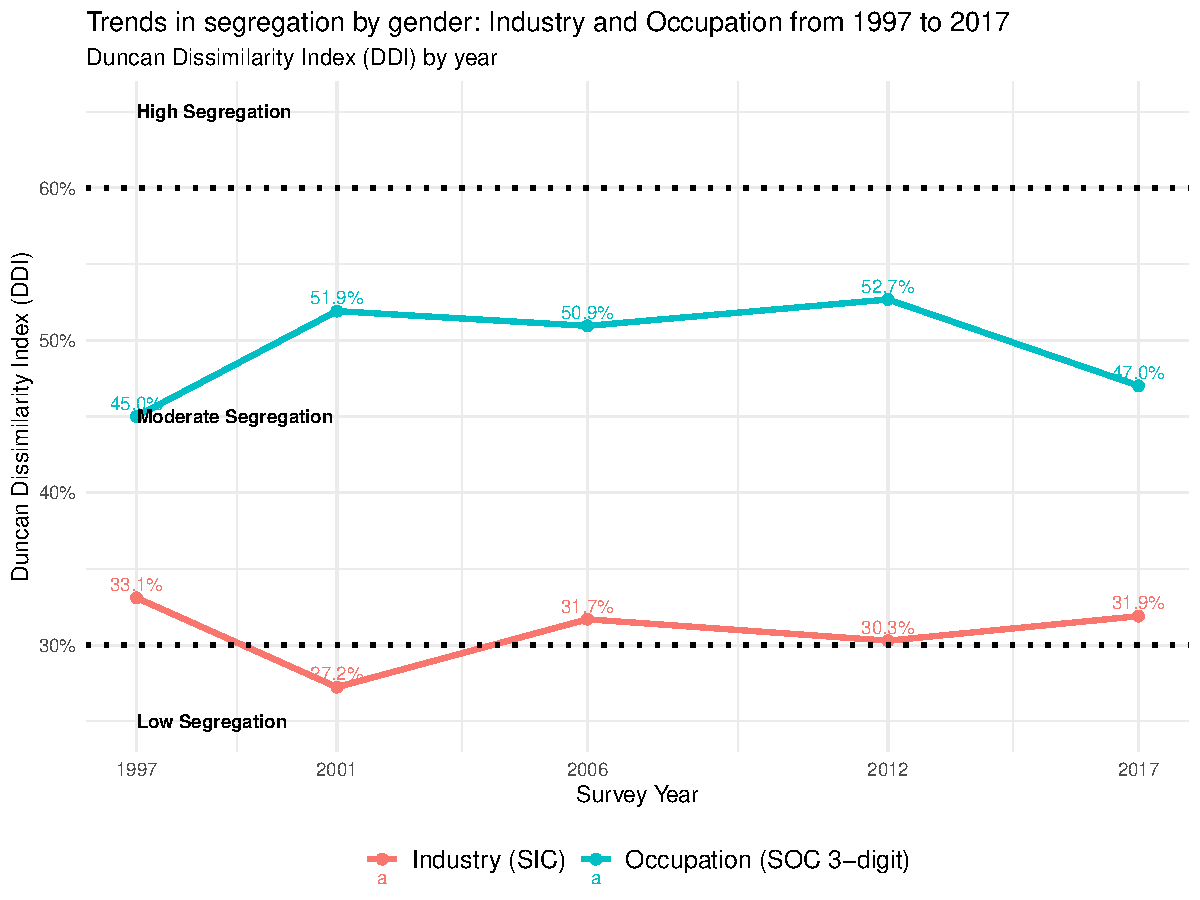
\includegraphics[width=\textwidth]{_graphic/industry_occupation3d_segreggation_fulltime.pdf}
    \label{fig:industry_occupation3d_segreggation_fulltime}
    \vspace{-3em}
    \justify\singlespacing\scriptsize\textit{Notes}: Notes here.
\end{figure}


The evolution of gender segregation in the UK labor market from 1997 to 2017 reveals persistent disparities
 in the distribution of men and women across both occupations and industries. Using the Duncan Dissimilarity 
 Index (D-index), I find that occupational segregation—measured at the 3-digit SOC level—remains consistently 
 moderate to high, with values ranging from 45.0\% in 1997 to 52.7\% in 2012, before declining slightly to 47.0\% 
 in 2017. These figures suggest that nearly half of either male or female workers would need to change occupations 
 to achieve gender parity, highlighting substantial and enduring occupational sorting by gender.

By contrast, industrial segregation—based on 2-digit SIC codes—remains lower and more stable, fluctuating 
between 27.2\% and 33.1\% over the same period. While both forms of segregation exhibit some variation, 
there is no strong or consistent trend toward greater integration over the 20-year span.

These results align with recent research documenting the persistence of occupational segregation despite 
broader gains in gender equality in education and employment. Studies such as England (2010), Blau and Kahn (2017), 
and Oesch et al. (2020) emphasize that, even as gender gaps in labor force participation and earnings have narrowed, 
occupational sorting continues to play a central role in maintaining inequality. Similarly, ILO (2021) and 
Rubery and Tavora (2020) note that gendered occupational patterns remain entrenched, even within high-skilled sectors. 
UK-specific analyses based on SES data (e.g., Green and Henseke, 2021) reinforce the view that occupational clustering 
and gendered task content have proven resilient. The higher and more variable levels of segregation observed at the 
occupational level underscore the value of disaggregated classifications such as 3-digit SOC codes in capturing 
structural barriers to gender integration.


\begin{table}[!t]
    \centering
    \caption{Task measures from the Skills and Employment Survey}
    \label{tab:task-ses}
    % \resizebox*{\textwidth}{!}{
    \begin{threeparttable}
        % \setlength{\tabcolsep}{6pt}
        % \small
        \begin{tabular}{@{}p{4cm}p{11cm}@{}}
    \toprule
    \textbf{Skill} & \textbf{Task} \\
    \midrule
    
    \multirow{6}{*}{Literacy} 
    & Reading written information, e.g.\ forms, notices, or signs \\
    & Reading short documents, e.g.\ letters or memos \\
    & Reading long documents, e.g.\ long reports, manuals, etc. \\
    & Writing material such as forms, notices, or signs \\
    & Writing short documents, e.g.\ letters or memos \\
    & Writing long documents with correct spelling/grammar \\
    
    \midrule
    \multirow{3}{*}{Numeracy} 
    & Adding, subtracting, multiplying, or dividing numbers \\
    & Calculations using decimals, percentages, or fractions \\
    & More advanced mathematical or statistical procedures \\
    
    \midrule
    \multirow{3}{*}{Numeracy} 
    & Adding, subtracting, multiplying, or dividing numbers \\
    & Calculations using decimals, percentages, or fractions \\
    & More advanced mathematical or statistical procedures \\

    \midrule
    \multirow{4}{*}{Physical} 
    & Carrying, pushing or pulling heavy objects \\
    & Working for long periods on physical activities \\
    & mend, repair, assemble, construct or adjust things \\
    & knowledge of how to use or operate tools, equipment or machinery \\

    \midrule
    \multirow{5}{*}{\begin{tabular}[c]{@{}l@{}}Professional\\ communication\end{tabular}} 
    & Instructing, training, or teaching people \\
    & Persuading or influencing others \\
    & Making speeches or presentations \\
    & Planning the activities of others \\
    & Listening carefully to colleagues \\
    
    \midrule
    \multirow{4}{*}{Problem solving} 
    & Spotting problems or faults \\
    & Working out the cause of problems or faults \\
    & Thinking of solutions to problems \\
    & Analysing complex problems in depth \\
    
    \midrule
    \multirow{6}{*}{\begin{tabular}[c]{@{}l@{}}Computer use\\ complexity\end{tabular}} 
    & Importance of computer use and complexity of computer use: \\
    & Not at all = 0 \\
    & Straightforward use = 1 \\
    & Moderate use = 2 \\
    & Complex use = 3 \\
    & Advanced use = 4 \\
    
    \bottomrule
    \end{tabular}



    
        \begin{tablenotes}[flushleft]
            \scriptsize{\item \textit{Source}: Adapted from \textcite{lindleyGenderDifferencesJob2015a}. 
            \item \textit{Notes}:Based on the factor analysis conducted in Green (2012).}
        \end{tablenotes}
    \end{threeparttable}
    % }
\end{table}






            


\section{Section} \label{sec:section}
\input{_chapter/02-section}

\section{Data and Methodology} \label{sec:methods1}

To capture gender segregation in the nature of work performed, I construct a \textit{task-based Dissimilarity Index}, denoted $D_{\text{task}}$. This measure extends the standard D index (typically applied to occupational or industry categories) to account for gender differences in task use across occupations.

Each respondent in the SES dataset reports the importance of 11 skill types in their job, using a scale from 0 to 4:

\begin{itemize}
    \item 0 = Does not apply in job
    \item 1 = Not very important
    \item 2 = Fairly important
    \item 3 = Very important
    \item 4 = Essential
\end{itemize}

To simplify the construction of a task use indicator, I convert each continuous skill score into a binary indicator, where a skill is considered used if its value exceeds 2.5:

\[
\text{TaskUsed}_{i,s} =
\begin{cases}
1 & \text{if } \text{Skill}_{i,s} > 2.5 \\
0 & \text{otherwise}
\end{cases}
\]

for individual $i$ and skill $s$. I then compute, for each occupation $j$ and skill $s$, the weighted share of men and women who report using the skill, using grossing weights $w_i = \text{gwtall}$. Let:

\begin{itemize}
    \item $M_{j,s}$ = weighted number of men in occupation $j$ using skill $s$
    \item $F_{j,s}$ = weighted number of women in occupation $j$ using skill $s$
    \item $T^M_j$, $T^F_j$ = total weighted men and women in occupation $j$
\end{itemize}

Then the task-level gender difference is:

\[
d_{j,s} = \left| \frac{M_{j,s}}{T^M_j} - \frac{F_{j,s}}{T^F_j} \right|
\]

If either gender is absent from occupation $j$, I assign $d_{j,s} = 1$, reflecting complete segregation.

I then compute the mean difference across all skills within occupation $j$:

\[
D_j = \frac{1}{S} \sum_{s=1}^{S} d_{j,s}
\]

where $S = 11$ is the number of skills. This yields an occupation-level segregation score $D_j \in [0, 1]$.

Finally, I compute the aggregate index in two forms:

\textbf{Unweighted average:}
\[
D_{\text{task}}^{\text{unweighted}} = \frac{1}{J} \sum_{j=1}^{J} D_j
\]

\textbf{Weighted average:}
\[
D_{\text{task}}^{\text{weighted}} = \sum_{j=1}^{J} \left( \frac{W_j}{\sum_{j=1}^{J} W_j} \right) D_j
\]

This index reflects the extent to which men and women perform different tasks across occupations, even when working in similar jobs or industries. 
It captures a dimension of gender segregation that is not visible through occupation or industry codes alone.

Figure X displays trends in gender task segregation across UK occupations from 1997 to 2017, measured using a 
modified version of the Duncan Dissimilarity Index. The figure distinguishes between an unweighted version of 
the index, which gives equal weight to each occupation, and a weighted version that adjusts for the employment 
size of occupations to reflect aggregate worker experience.

The unweighted index reveals persistently moderate levels of task segregation, with values ranging from 52.7% 
in 1997 to 46.5\% in 2017. Although there is an overall decline across the two decades, the pattern is non-linear, 
with a noticeable dip in 2006 followed by a rebound in 2012. This suggests that the degree of task differentiation 
between men and women within occupations remains substantial and relatively stable when each occupation is treated 
equally, regardless of size.

By contrast, the weighted index—which accounts for the number of individuals employed in each occupation—shows a 
consistently lower level of task segregation, ranging from 36.9\% in 2006 to 34.8\% in 2012, and ending at 32.2% in 
2017. This indicates that the average worker in the labour market experiences significantly lower task segregation 
than the unweighted average suggests, implying that larger occupations tend to exhibit more gender-integrated task 
profiles.

The divergence between the weighted and unweighted trends underscores the importance of accounting for employment 
size when assessing the extent of gender segregation. While smaller occupations may exhibit higher levels of gendered 
task differentiation, they employ fewer individuals and therefore contribute less to aggregate patterns. The weighted 
index suggests a modest downward trend in task segregation over time, albeit from already relatively low levels. 
Together, these findings point to a persistent but gradually declining pattern of gender-based task differentiation 
within occupations, with significant variation across the occupational structure.

\begin{figure}[!t]
    \centering
    \caption{Task Seggregation}
    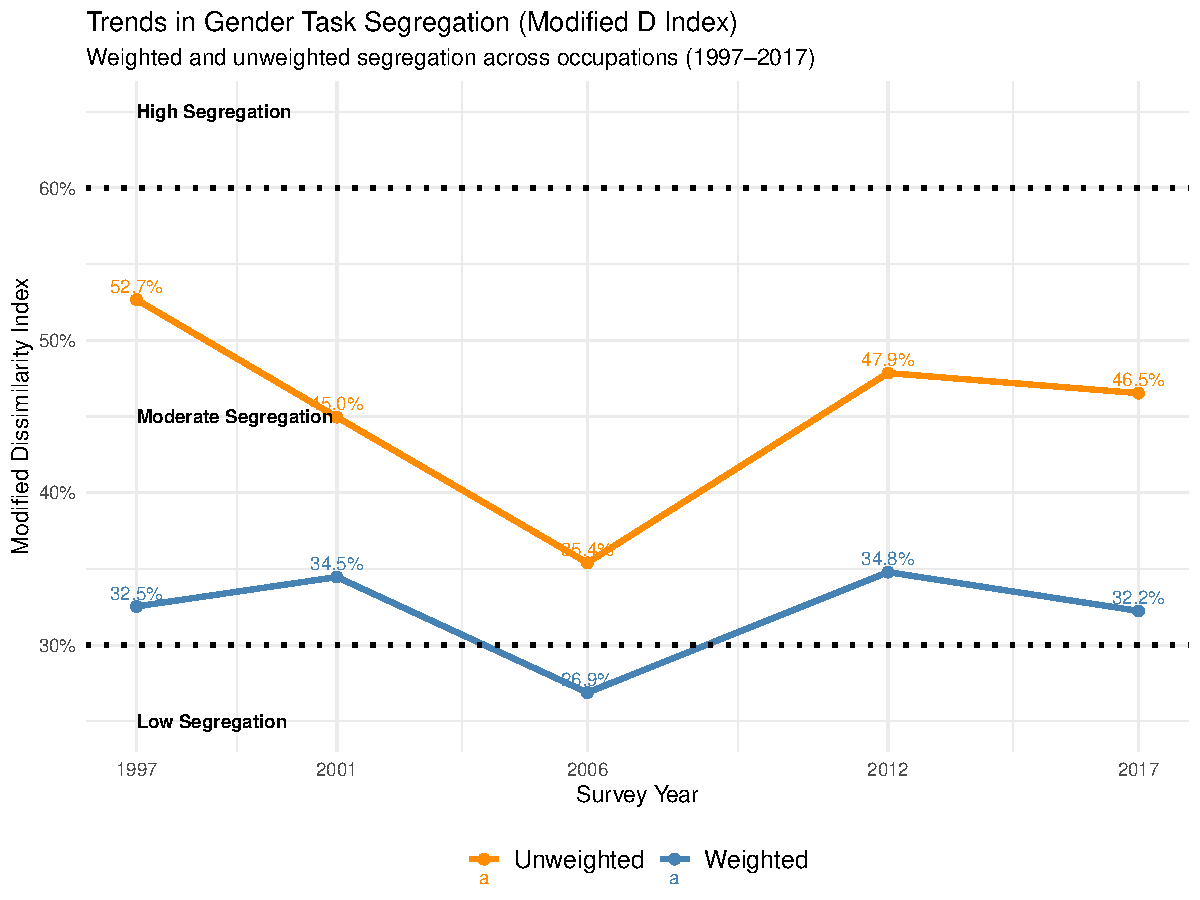
\includegraphics[width=\textwidth]{_graphic/task_segregation.pdf}
    \label{fig:task_segregation}
    \vspace{-3em}
    \justify\singlespacing\scriptsize\textit{Notes}: Notes here.
\end{figure}



\begin{figure}[!t]
    \centering
    \caption{Title}
    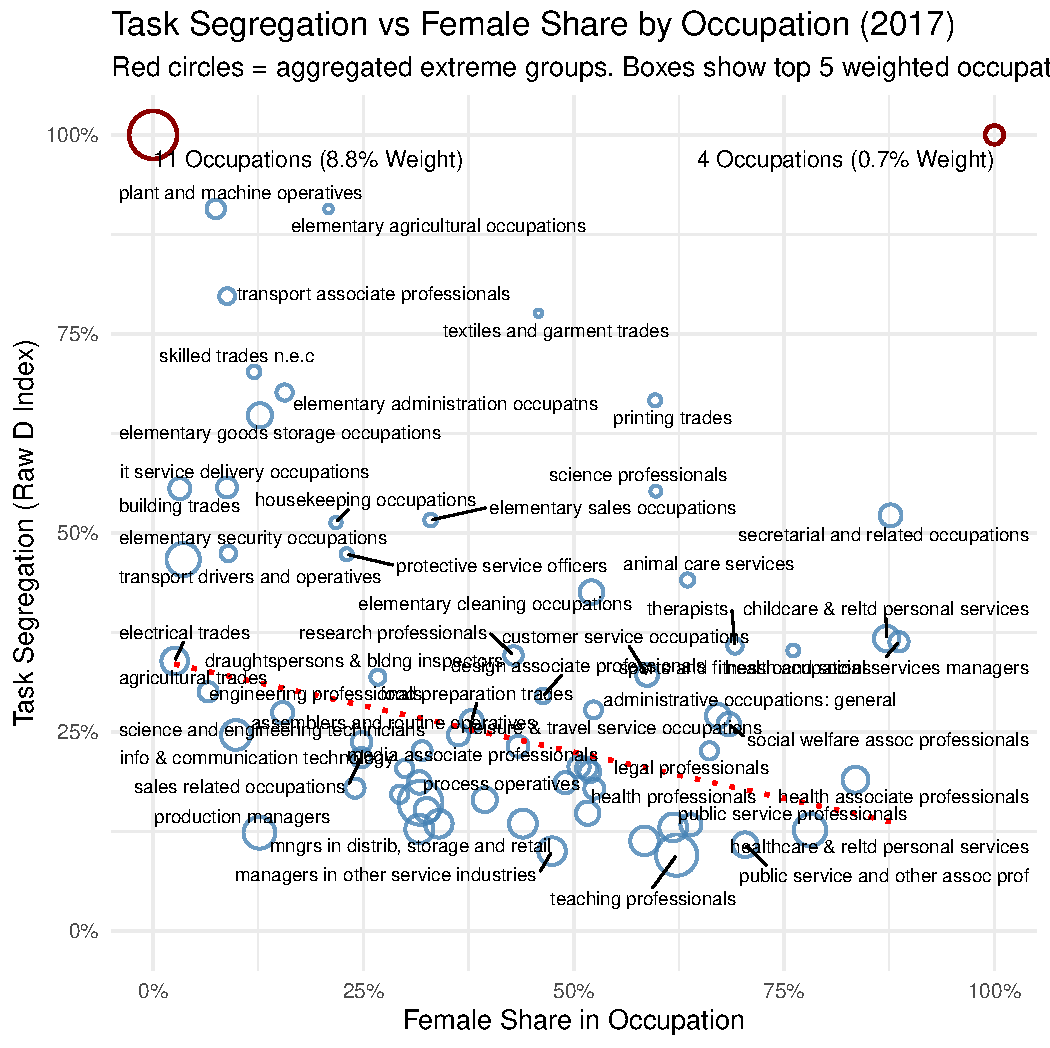
\includegraphics[width=\textwidth]{_graphic/task_b3occ_females_share_nobox.pdf}
    \label{fig:task_b3occ_females_share_nobox}
    \vspace{-3em}
    \justify\singlespacing\scriptsize\textit{Notes}: Notes here.
\end{figure}

The scatter plot illustrates the relationship between task segregation and female occupational share 
in the UK labour market in 2017. Each point represents a 3-digit SOC occupation, with task segregation 
measured by the modified D on the vertical axis and the proportion of women in each occupation 
on the horizontal axis. A negative association emerges: occupations with a higher share of women 
tend to exhibit lower levels of task segregation, suggesting that in more gender-balanced or female-dominated 
roles, men and women are more likely to perform similar tasks. This pattern is captured by the downward-sloping 
trend line, indicating that gender-based task differentiation diminishes as female representation increases.

However, beyond this general trend, a number of occupations lie well above the trend line, indicating 
significantly higher levels of task segregation than would be predicted based on their gender composition 
alone. These outliers are concentrated in both male- and female-dominated fields, revealing that high task 
segregation is not confined to one side of the gender distribution. On the male-dominated side, occupations 
such as plant and machine operatives, transport associate professionals, and skilled trades (not elsewhere classified) 
display relatively high levels of task segregation, even after accounting for their low female share. 
On the female-dominated side, occupations such as textiles and garment trades, printing trades, and science 
professionals also show elevated levels of task segregation despite having moderate to high female representation.

These patterns suggest that in some occupations, the division of tasks between men and women is especially 
pronounced. In these cases, gendered role 
expectations or organizational structures may contribute to sharp internal task differentiation. 
Such deviations from the average pattern highlight the importance of examining within-occupation task 
segregation directly, rather than relying solely on measures of occupational gender composition, in order 
to uncover the mechanisms through which gendered labour market inequalities are maintained.

\section{Gender Wage Gap} \label{sec:methods2}

The empirical analysis estimates the gender wage gap using the following log-linear regression model:

\begin{equation}
\log(wage_i) = \alpha + \beta \cdot Female_i + \mathbf{X}_i'\boldsymbol{\gamma} + \delta_{j(i)} + \theta_{k(i)} + \varepsilon_i
\end{equation}

where $\log(wage_i)$ denotes the natural logarithm of hourly wages for individual $i$, and $Female_i$ is a binary 
indicator equal to one if the individual is female and zero otherwise. The vector $\mathbf{X}_i$ includes individual-level 
controls such as age, education, and region. The terms $\delta_{j(i)}$ and $\theta_{k(i)}$ represent fixed effects for occupation 
(3-digit SOC) and industry (2-digit SIC), respectively, and $\varepsilon_i$ is the error term. In extended specifications, the model 
incorporates additional variables capturing task and skill requirements derived from job-level data. The coefficient $\beta$ measures 
the conditional gender wage gap, interpreted as the average percentage difference in hourly wages between women and men, conditional 
on observed characteristics, occupational sorting, and task content.


Table X reports estimates of the gender wage gap from a series of linear regressions where the 
dependent variable is the log of hourly wages. Column (1) presents the baseline specification, 
which includes controls for individual-level characteristics such as age, education, and region. 
In this model, women earn approximately 14.9\% less than men. Column (2) adds controls for occupation and industry, reducing the estimated wage 
gap to 6.1\% and explaining 59.2\% of the initial difference. This substantial reduction highlights the 
central role of occupational and industrial sorting in shaping gender disparities in pay.

Columns (3) through (14) sequentially introduce a wide range of skill and task measures, including 
indicators of cognitive, manual, interpersonal, and planning-related demands. Across these models, 
the adjusted gender wage gap remains consistently between 5.4\% and 7.4\%, with relatively minor variation 
in the percent of the gap explained. The highest explanatory power is reached in column (12), where 63.6\% of 
the original gap is accounted for, while the lowest occurs in column (13), at 50.6\%. These changes, though 
measurable, are modest compared to the explanatory contribution of occupation and industry introduced in column (2).

Overall, the results suggest that while gender differences in task and skill requirements explain a small 
additional portion of the wage gap, the vast majority of the explained component derives from gender sorting 
into different occupations and industries. Even after accounting for detailed task characteristics, a 
persistent and statistically significant wage penalty of around 6\% remains for women, pointing to the 
enduring role of within-job and potentially discriminatory mechanisms in the gender wage structure.

\begin{table}[!t]
    \centering
    \caption{Gender Wage Gap}
    \label{tab:task-wagegap}
     \resizebox*{\textwidth}{!}{
    \begin{threeparttable}
        % \setlength{\tabcolsep}{6pt}
        % \small
        \begin{tabular}{@{}p{3.8cm}cccccccccccccc@{}}
    \toprule
     & (1) & (2) & (3) & (4) & (5) & (6) & (7) & (8) & (9) & (10) & (11) & (12) & (13) & (14) \\
    \midrule
    Female & -0.149*** & -0.061* & -0.063* & -0.060* & -0.059* & -0.064* & -0.056* & -0.060* & -0.061* & -0.061* & -0.064* & -0.054+ & -0.074** & -0.064* \\
           & (0.026)   & (0.028) & (0.028) & (0.028) & (0.028) & (0.028) & (0.027) & (0.028) & (0.028) & (0.028) & (0.027) & (0.029) & (0.027) & (0.028) \\
    Individual controls & Yes & Yes & Yes & Yes & Yes & Yes & Yes & Yes & Yes & Yes & Yes & Yes & Yes & Yes \\
    Occupation and Industry     & No  & Yes & Yes & Yes & Yes & Yes & Yes & Yes & Yes & Yes & Yes & Yes & Yes & Yes \\
    \% Gender Gap Explained                 & 0\% & 59.2\% & 57.6\% & 59.5\% & 60.4\% & 57.1\% & 62.4\% & 59.9\% & 59.1\% & 59.2\% & 57.3\% & 63.6\% & 50.6\% & 56.8\% \\
    Observations                            & 16,735,292 & 16,735,292 & 16,735,292 & 16,735,292 & 16,735,292 & 16,735,292 & 16,735,292 & 16,735,292 & 16,735,292 & 16,735,292 & 16,735,292 & 15,821,040 & 16,735,292 & 15,821,040 \\
    \bottomrule
    \end{tabular}
    
        \begin{tablenotes}[flushleft]
            \scriptsize{\item \textit{Source}: Adapted from \textcite{lindleyGenderDifferencesJob2015a}. 
            \item \textit{Notes}: Stadardt errors are clustered at the occupation level. + p < 0.1, * p < 0.05, ** p < 0.01, *** p < 0.001.}
        \end{tablenotes}
    \end{threeparttable}
     }
\end{table}


\section{Conclusion} \label{sec:conclusion}
We may have reached the conclusion too quickly.

\begin{table}[!t]
    \centering
    \caption{Occupations characteristics from the O*NET database}
    \label{tab:task-onet}
     \resizebox*{0.7\textwidth}{!}{
    \begin{threeparttable}
        % \setlength{\tabcolsep}{6pt}
        % \small
            \begin{tabular}{@{}p{4cm}p{11cm}@{}}
    \toprule
    \textbf{Construct} & \textbf{Based on Questions from Job Surveys} \\
    \midrule
    
    \textit{Competition} & “How competitive is your current job?” \\
    
    \midrule
    \textit{Social Contribution} & 
    \begin{itemize}
      \item “How important is concern for others to the performance of your current job?”
      \item “How important is assisting and caring for others to the performance of your current job?”
      \item “How important is service orientation to the performance of your current job?” (actively looking for ways to help people)
    \end{itemize} \\
    
    \midrule
    \textit{Inflexibility} & 
    \begin{itemize}
      \item “How often does your current job require you to meet strict deadlines?”  
      \newline (1: never, 2: once a year or more but not every month, 3: once a month or more but not every week, 4: once a week or more but not every day, 5: every day)
      \item “How many hours do you work in a typical week on your current job?”  
      \newline (1: less than forty hours, 2: forty hours, 3: more than forty hours)
    \end{itemize} \\
    
    \midrule
    \textit{Interactional Skills} & 
    \begin{itemize}
      \item “How much contact with others (by telephone, face to face, or otherwise) is required to perform your current job?”
      \item “How important are interactions that require you to work with or contribute to a work group or team to perform your current job?”
      \item “How important is establishing and maintaining interpersonal relationships to the performance of your current job?”
      \item “How important is social perceptiveness to the performance of your current job?”
    \end{itemize} \\
    
    \midrule
    \textit{Cognitive Skills} & 
    \begin{itemize}
      \item Written comprehension
      \item Mathematical reasoning ability
      \item Deductive reasoning
      \item Inductive reasoning
    \end{itemize} \\
    
    \midrule
    \textit{Physical Skills} & 
    \begin{itemize}
      \item General physical activities
      \item Handling and moving objects
    \end{itemize} \\
    \bottomrule
    \end{tabular}

    
        \begin{tablenotes}[flushleft]
            \scriptsize{\item \textit{Source}: Adapted from \textcite{cortes2018occupation}}
        \end{tablenotes}
    \end{threeparttable}
     }
\end{table}

\begin{table}[htbp]
    \centering
    \caption{\textit{Table A1.} \quad O*NET 13.0 -- Work Activities \& Work Context.}
    \label{tab:task-onet-autom}
    \begin{threeparttable}
        \begin{tabular}{@{}ll@{}}
    \toprule
    \multicolumn{2}{l}{\textbf{A. Characteristics Linked to Technological Change/Offshorability}} \\
    \midrule
    \multicolumn{2}{l}{\textit{Information Content}} \\
    4.A.1.a.1   & Getting Information (JK) \\
    4.A.2.a.2   & Processing Information (JK) \\
    4.A.2.a.4   & Analyzing Data or Information (JK) \\
    4.A.3.b.1   & Interacting with Computers (JK) \\
    4.A.3.b.6   & Documenting/Recording Information (JK) \\
    
    \addlinespace
    \multicolumn{2}{l}{\textit{Automation/Routinization}} \\
    4.C.3.b.2   & Degree of Automation \\
    4.C.3.b.7   & Importance of Repeating Same Tasks \\
    4.C.3.b.8   & Structured versus Unstructured Work (reverse) \\
    4.C.3.d.3   & Pace Determined by Speed of Equipment \\
    4.C.2.d.1.i & Spend Time Making Repetitive Motions \\
    
    \midrule
    \multicolumn{2}{l}{\textbf{B. Characteristics Linked to Non-Offshorability}} \\
    \midrule
    \multicolumn{2}{l}{\textit{Face-to-Face}} \\
    4.C.1.a.2.l & Face-to-Face Discussions \\
    4.A.4.a.4   & Establishing and Maintaining Interpersonal Relationships (JK,B) \\
    4.A.4.a.5   & Assisting and Caring for Others (JK,B) \\
    4.A.4.a.8   & Performing for or Working Directly with the Public (JK,B) \\
    4.A.4.b.5   & Coaching and Developing Others (B) \\
    
    \addlinespace
    \multicolumn{2}{l}{\textit{On-Site Job}} \\
    4.A.1.b.2   & Inspecting Equipment, Structures, or Material (JK) \\
    4.A.3.a.2   & Handling and Moving Objects \\
    4.A.3.a.3   & Controlling Machines and Processes \\
    4.A.3.a.4   & Operating Vehicles, Mechanized Devices, or Equipment \\
    4.A.3.b.4   & Repairing and Maintaining Mechanical Equipment (*0.5) \\
    4.A.3.b.5   & Repairing and Maintaining Electronic Equipment (*0.5) \\
    
    \addlinespace
    \multicolumn{2}{l}{\textit{Decision Making}} \\
    4.A.2.b.1   & Making Decisions and Solving Problems (JK) \\
    4.A.2.b.2   & Thinking Creatively (JK) \\
    4.A.2.b.4   & Developing Objectives and Strategies \\
    4.C.1.c.2   & Responsibility for Outcomes and Results \\
    4.C.3.a.2.b & Frequency of Decision Making \\
    
    \bottomrule
    \end{tabular}

    
    \begin{tablenotes}[flushleft]
    \scriptsize
    \item \textit{Source:} Adapted from \textcite{fortinInequalityChangesTask2016}
    \item \textit{Notes:} (JK) indicates a work activity used in Jensen and Kletzer (2007), (B) a work activity used or suggested in Blinder (2007).
\end{tablenotes}
    \end{threeparttable}
    \end{table}
    

    \begin{table}[htbp]
        \centering
        \caption{Classification of tasks Germany}
        \label{tab:task-onet-germany}
        \resizebox*{\textwidth}{!}{
        \begin{threeparttable}
             \begin{tabular}{@{}ll@{}}
    \toprule
    \textbf{Category} & \textbf{Tasks} \\
    \midrule
    Abstract tasks & calculating and correcting text/data; executing, interpreting, and advising on law/rules; planning, projecting, and designing; programming; researching, analysing, and evaluating \\
    \addlinespace
    Interactive tasks & advertising, publishing, and public relations; coordinating and organising; negotiating and advising; teaching and training \\
    \addlinespace
    Manual tasks & repairing, restoring, and renovating; securing; serving and accommodating guests \\
    \addlinespace
    Routine tasks & cleaning and rubbish removal; equipping and operating machinery; manufacturing or producing; measuring length/weight/temperature \\
    \bottomrule
    \end{tabular}

    
        \begin{tablenotes}[flushleft]
        \scriptsize
        \item \textit{Source:} Adapted from \textcite{miriamkoomenOccupationalTasksWage2022}
        \item \textit{Notes:} 
    \end{tablenotes}
        \end{threeparttable}
        }
        \end{table}
          

        \begin{table}[htbp]
            \centering
            \caption{Major Occupational and Industry Classification Systems (Latest Versions)}
            \label{tab:task-classification}
            \resizebox*{\textwidth}{!}{
            \begin{threeparttable}
                    \begin{tabular}{@{}p{7cm}p{2.5cm}p{4cm}p{10cm}@{}}
    \toprule
    \textbf{Name} & \textbf{Abbreviation} & \textbf{Country / Organization} & \textbf{Details} \\
    \midrule
    
    Standard Occupational Classification & SOC2010 & UK (ONS) & Latest UK occupational classification; 4-digit structure; used in SES2017 and LFS. \\
    \addlinespace
    International Standard Classification of Occupations & ISCO08 & International Labour Organization (ILO) & Global occupation classification for international comparison; 4-tier hierarchy. \\
    \addlinespace
    Standard Industrial Classification  & SIC2007 & UK (ONS) & Current UK industry coding system based on NACE Rev. 2; used for business and labor statistics. \\
    \addlinespace
    National Statistics Socio-Economic Classification  & NS-SEC2010 & UK (ONS) & Socio-economic class measure based on occupation (e.g. managerial, routine); based on SOC2010. \\
    \addlinespace
    Occupational Information Network & O*NET & U.S. (Department of Labor) & U.S. occupational database linking SOC codes to tasks, skills, work context, etc.; widely used in job-task research. \\
    \addlinespace
    European Skills, Competences, Qualifications and Occupations & ESCO & EU (European Commission) & European job and skill classification; aligned with ISCO08; used for labor mobility and training. \\
    
    \bottomrule
    \end{tabular}

    
            \begin{tablenotes}[flushleft]
            \scriptsize
            \item \textit{Source:} Author own elaboration.
            \item \textit{Notes:} 
        \end{tablenotes}
            \end{threeparttable}
            }
            \end{table}
              

%% Comments the lines below
% \clearpage
% \section{New material}
% \input{_chapter/99-newmaterial}

\clearpage
\onehalfspacing % Bibliography and appendix in one half spacing

%\bibliographystyle{apalike}
\printbibliography


%%% APPENDIX %%%
\clearpage
\appendix
\section*{Appendices}
\addcontentsline{toc}{section}{Appendices}
\renewcommand{\thesubsection}{\Alph{subsection}}
\counterwithin{figure}{subsection}
\counterwithin{table}{subsection}
\renewcommand\thefigure{\thesubsection.\arabic{figure}}
\renewcommand{\thetable}{\thesubsection.\arabic{table}}

\subsection{Appendix A}\label{app-A}
\input{_chapter/A-appendix}
\clearpage
\subsection{Appendix B}\label{app-B}
\input{_chapter/B-appendix}

\counterwithout{figure}{subsection}
\counterwithout{table}{subsection}

%%%%% ADDITIONAL APPENDICES %%%%
% `\nolink` removes links to literature in online and review appendix
\newcommand*{\nolink}[1]{%
  {\protect\NoHyper#1\protect\endNoHyper}%
}
% To remove links to equation or section, use `\ref*` instead of `\ref`

%%% ONLINE APPENDIX %%%
\clearpage
\begin{center}
    \section*{Online Appendix}
    \addcontentsline{toc}{section}{Online Appendix}
    \textbf{\Large \thetitle}\\
    \vspace{1em}
    \theauthor
\end{center}
\vspace{1em}

% Short name of the section
\renewcommand{\thesection}{OA}

% Setup for pages, figures, and tables
\pagenumbering{arabic}% resets `page` counter to 1
\renewcommand{\thepage}{\thesection-\arabic{page}}
\counterwithin{figure}{section}
\counterwithin{table}{section}
\setcounter{figure}{0} % resets `figure` counter to 1
\setcounter{table}{0} % resets `table` counter to 1
\renewcommand{\thefigure}{\thesection.\arabic{figure}}
\renewcommand{\thetable}{\thesection.\arabic{table}}

\input{_chapter/O-online}

%%% REVIEWER APPENDIX %%%
\clearpage
\begin{center}
    \section*{Reviewer Appendix}
    \addcontentsline{toc}{section}{Reviewer Appendix}
    \textbf{\Large \thetitle}\\
    \vspace{1em}
    \theauthor
\end{center}
\vspace{1em}

% Short name of the section
\renewcommand{\thesection}{RA}

% Setup for pages, figures, and tables
\pagenumbering{arabic}% resets `page` counter to 1
\renewcommand{\thepage}{\thesection-\arabic{page}}
\counterwithin{figure}{section}
\counterwithin{table}{section}
\setcounter{figure}{0} % resets `figure` counter to 1
\setcounter{table}{0} % resets `table` counter to 1
\renewcommand{\thefigure}{\thesection.\arabic{figure}}
\renewcommand{\thetable}{\thesection.\arabic{table}}

\input{_chapter/R-reviewer}

%%% PERSONAL APPENDIX %%%
%\clearpage
%\begin{center}
%   \section*{Personal Appendix}
%    \addcontentsline{toc}{section}{Personal Appendix}
%    \textbf{\Large \thetitle}\\
%    \vspace{1em}
%    \theauthor
%\end{center}
%\vspace{1em}

%% Short name of the section
%\renewcommand{\thesection}{PA}

%% Setup for pages, figures, and tables
%\pagenumbering{arabic}% resets `page` counter to 1
%\renewcommand{\thepage}{\thesection-\arabic{page}}
%\counterwithin{figure}{section}
%\counterwithin{table}{section}
%\setcounter{figure}{0} % resets `figure` counter to 1
%\setcounter{table}{0} % resets `table` counter to 1
%\renewcommand{\thefigure}{\thesection.\arabic{figure}}
%\renewcommand{\thetable}{\thesection.\arabic{table}}

%\input{_chapter/P-personal}

\end{document}